\subsection{三角形全等的判定 I}\label{subsec:czjh1-3-5}

根据定义来判定两个三角形全等,需要知道三条边对应相等和三个角对应相等。
现在我们来研究是否可以减少一些条件,找到比较简单的判定方法。
为此,我们先举例说明如何画出满足一定条件的三角形。

用刻度尺和量角器,画一个三角形,使它的两条边长分别是 2.8 cm 和 3.1 cm,
这两条边的夹角等于 $45^\circ$。

\huafa 1. 画 $\angle DAE = 45^\circ$ (图 \ref{fig:czjh1-3-16})。

2. 在 $AD$、$AE$ 上分别截取 $AB = 3.1\;\limi$, $AC = 2.8\;\limi$。

3. 连结 $BC$。

$\triangle ABC$ 就是所求的三角形。

\begin{figure}[htbp]
    \centering
    \begin{minipage}[b]{4.5cm}
        \centering
        \begin{tikzpicture}
    \tkzDefPoints{0/0/A, 3.1/0/B, 3.5/0/D}
    \tkzDefPoint(45:2.8){C}
    \tkzDefPointOnLine[pos=1.3](A,C)  \tkzGetPoint{E}

    \tkzDrawSegments(A,D  A,E  B,C)
    \tkzLabelPoints[above](E)
    \tkzLabelPoints[left](C)
    \tkzLabelPoints[below](A,B)
    \tkzLabelPoints[right](D)
\end{tikzpicture}


        \caption{}\label{fig:czjh1-3-16}
    \end{minipage}
    \qquad
    \begin{minipage}[b]{9cm}
        \centering
        \begin{tikzpicture}
    % 两个 scope 的区别,仅仅在于各点的名称不同。
    % 所以将绘制代码抽取出来(复用)
    \def\drawtriangle{
        \tkzDefPoints{0/0/B, 3.5/0/C, 2.8/2/A}
        \tkzDrawPolygon(A,B,C)
        \tkzMarkSegment[mark=|](A,B)
        \tkzMarkSegment[mark=||](A,C)
        \tkzMarkAngle[size=0.3](B,A,C)
    }

    \begin{scope}
        \drawtriangle
        \tkzLabelPoints[above](A)
        \tkzLabelPoints[below](B,C)
    \end{scope}

    \begin{scope}[xshift=4.5cm]
        \drawtriangle
        \tkzLabelPoint[above](A){$A'$}
        \tkzLabelPoint[below](B){$B'$}
        \tkzLabelPoint[below](C){$C'$}
    \end{scope}
\end{tikzpicture}


        \caption{}\label{fig:czjh1-3-17}
    \end{minipage}
\end{figure}

如果按照上面的条件,用同样的方法另画一个 $\triangle A'B'C'$,
再把 $\triangle A'B'C'$ 剪下来放到 $\triangle ABC$ 上,我们可以看到,
$\triangle A'B'C'$ 与 $\triangle ABC$ 能够完全重合。
这个事实说明,只要是按上述条件画出的三角形,它们总是全等的。我们把这个事实作为公理:

\begin{gongli}[边角边公理]
    有两边和它们的夹角对应相等的两个三角形全等
\end{gongli}(可以简写成 “\zhongdian{边角边}” 或 “$\bm{SAS}$”)。

例如,在图 \ref{fig:czjh1-3-17} 的 $\triangle ABC$ 和 $\triangle A'B'C'$ 中,
如果 $AB = A'B'$, $\angle A = \angle A'$, $AC = A'C'$, 那么
$$ \triangle ABC \quandeng \triangle A'B'C' \juhao $$

根据边角边公理可以判定两个三角形全等。


\liti 已知: $AD \pingxing BC$, $AD = CB$ ( 图 \ref{fig:czjh1-3-18})。

求证: $\triangle ADC \quandeng CBA$。

\zhengming $\because$ \quad $AD \pingxing BC$ (已知),

$\therefore$ \quad $\angle 1 = \angle 2$ (两直线平行,内错角相等)。

在 $\triangle ADC$ 和 $\triangle CBA$ 中,

\hspace{2em}$\begin{cases}
    AD = CB \quad \text{(已知),} \\
    \angle 1 = \angle 2  \quad \text{(已证),} \\
    AC = CA  \quad \text{(公共边),} \\
\end{cases}$

$\therefore$ \quad $\triangle ADC \quandeng \triangle CBA$ ($SAS$)。


\begin{figure}[htbp]
    \centering
    \begin{minipage}[b]{7cm}
        \centering
        \begin{tikzpicture}
    \tkzDefPoints{0/0/B, 3/0/C, -0.7/2.0/A, 2.3/2.0/D}

    \tkzDrawPolygon(A,B,C,D)
    \tkzDrawSegments(A,C)
    \tkzMarkAngles[size=0.6](C,A,D  A,C,B)
    \tkzLabelAngle[pos=0.9](C,A,D){$1$}
    \tkzLabelAngle[pos=0.9](A,C,B){$2$}
    \tkzLabelPoints[left](A,B)
    \tkzLabelPoints[right](D,C)
\end{tikzpicture}


        \caption{}\label{fig:czjh1-3-18}
    \end{minipage}
    \qquad
    \begin{minipage}[b]{7cm}
        \centering
        \begin{tikzpicture}
    \tkzDefPoints{0/0/D, 1.8/0/A, 2.5/3.0/B}
    \tkzDefPointBy[rotation=center A angle -20](D)  \tkzGetPoint{E}
    \tkzDefPointBy[rotation=center A angle -20](B)  \tkzGetPoint{C}

    \tkzDrawPolygon(D,A,B)
    \tkzDrawPolygon(E,A,C)
    \tkzMarkAngles[size=0.6](E,A,D  C,A,B)
    \tkzLabelAngle[pos=1.0](E,A,D){$1$}
    \tkzLabelAngle[pos=1.0](C,A,B){$2$}
    \tkzLabelPoints[left](E,D)
    \tkzLabelPoints[right](A,C)
    \tkzLabelPoints[above](B)
\end{tikzpicture}


        \caption{}\label{fig:czjh1-3-19}
    \end{minipage}
\end{figure}

\liti 已知:如图 \ref{fig:czjh1-3-19}, $AB = AC$, $AD = AE$, $\angle 1 = \angle 2$。

求证: $\triangle ABD \quandeng \triangle ACE$。

\zhengming $\because$ \quad $\angle 1 = \angle 2$ (已知),

$\therefore$ \quad $\angle 1 + \angle EAB = \angle 2 + \angle EAB$ (等式的性质),

即  $\angle DAB = \angle EAC$。

在 $\triangle ABD$ 和 $\triangle ACE$ 中,

\hspace{2em}$\begin{cases}
    AB = AC \quad \text{(已知),} \\
    \angle DAB = \angle EAC \quad \text{(已证),} \\
    AD = AE \quad \text{(已知),} \\
\end{cases}$

$\therefore$ \quad $\triangle ABD \quandeng \triangle ACE$ ($SAS$)。


\begin{lianxi}

\xiaoti{已知:如图, $AB$ 和 $CD$ 相交于点 $E$, $EA = EC$, $ED = EB$。\\
    求证: $\triangle AED \quandeng \triangle CEB$。
}

\begin{figure}[htbp]
    \centering
    \begin{minipage}[b]{7cm}
        \centering
        \begin{tikzpicture}
    \tkzDefPoints{0/0/C, 0.8/1.2/E}
    \tkzDefPointBy[rotation=center E angle -100](C)  \tkzGetPoint{A}
    \tkzDefPointOnLine[pos=2.5](A,E)  \tkzGetPoint{B}
    \tkzDefPointOnLine[pos=2.5](C,E)  \tkzGetPoint{D}

    \tkzDrawPolygon(A,E,D)
    \tkzDrawPolygon(C,E,B)
    \tkzLabelPoints[left](A,C)
    \tkzLabelPoints[right](B,D,E)
\end{tikzpicture}


        \caption*{(第 1 题)}
    \end{minipage}
    \qquad
    \begin{minipage}[b]{7cm}
        \centering
        \begin{tikzpicture}
    \tkzDefPoints{0/0/B, 3/0/C,  1.5/3/A}
    \tkzDefMidPoint(A,B)  \tkzGetPoint{F}
    \tkzDefMidPoint(A,C)  \tkzGetPoint{E}

    \tkzDrawSegments(A,B  A,C  B,E  C,F)
    \tkzLabelPoints[above](A)
    \tkzLabelPoints[below](B,C)
    \tkzLabelPoints[left](F)
    \tkzLabelPoints[right](E)
\end{tikzpicture}


        \caption*{(第 2 题)}
    \end{minipage}
\end{figure}


\xiaoti{已知:如图,$AB = AC$, $F$、$E$ 分别是 $AB$、$AC$ 的中点。\\
    求证: $\triangle ABE \quandeng \triangle ACF$。
}

\end{lianxi}




\liti 如图 \ref{fig:czjh1-3-20}, 有一池塘。要测池塘两端 $A$、$B$ 的距离,
可先在平地上取一个可以直接到达 $A$ 和 $B$ 的点 $C$,
连结 $AC$ 并延长到 $D$,使 $CD = CA$。
连结 $BC$ 并延长到 $E$,使 $CE = CB$。
连结 $DE$,那么量出 $DE$ 的长,就是 $A$、$B$ 的距离。为什么?
按图写出 “已知” 、“求证”,并证明。

已知:$AD$ 与 $BE$ 交于点 $C$,  $CA = CD$, $CB = CE$。

求证:$AB = DE$。

\zhengming 在 $\triangle ACB$ 和 $\triangle DCE$ 中,

\hspace{2em}$\begin{cases}
    CA = CD \quad \text{(已知),} \\
    \angle 1 = \angle 2 \quad \text{(对顶角相等),} \\
    CB = CE \quad \text{(已知),} \\
\end{cases}$

$\therefore$ \quad $\triangle ACB \quandeng \triangle DCE$  ($SAS$)。

$\therefore$ \quad $AB = DE$ (全等三角形的对应边相等)。

\begin{figure}[htbp]
    \centering
    \begin{minipage}[b]{7cm}
        \centering
        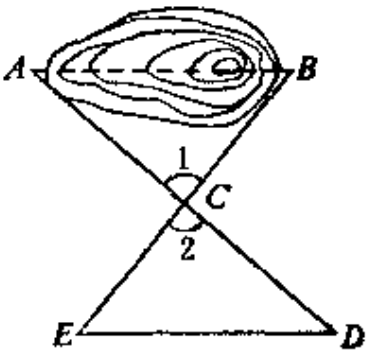
\includegraphics[width=5cm]{../pic/czjh1-ch3-20.png}
        \caption{}\label{fig:czjh1-3-20}
    \end{minipage}
    \qquad
    \begin{minipage}[b]{7cm}
        \centering
        \begin{tikzpicture}
    \tkzDefPoints{0/0/A, 2/0/B,  2.5/0/C, 4.5/0/D, 0/1.5/E, 4.5/-1.5/F}

    \tkzDrawSegments(A,D  A,E  B,E  C,F  D,F)
    \tkzMarkRightAngle(E,A,B)
    \tkzMarkRightAngle(C,D,F)
    \tkzLabelPoints[above](E,C,D)
    \tkzLabelPoints[below](A,B,F)
\end{tikzpicture}


        \caption*{(第 1 题)}
    \end{minipage}
\end{figure}


因为全等三角形的对应边、对应角相等,所以,
证明分别属于两个三角形的线段相等或者角相等的问题,
可以通过证明这两个三角形全等来解决。


\begin{lianxi}

\xiaoti{已知:如图,点 $A$、$B$、$C$、$D$ 在同一条直线上, $AC = DB$, $AE = DF$,
    $EA \perp AD$, $FD \perp AD$,垂足分别是 $A$、$D$。\\
    求证: $\triangle EAB \quandeng \triangle FDC$。
}


\xiaoti{已知:如图,点 $E$、$F$ 在 $BC$ 上, $BE = CF$, $AB = DC$, $\angle B = \angle C$。\\
    求证: $AF = DE$。
}

\begin{figure}[htbp]
    \centering
    \begin{minipage}[b]{7cm}
        \centering
        \begin{tikzpicture}
    \tkzDefPoints{0/0/B, 0.8/0/E,  3.2/0/F, 4/0/C}
    \tkzDefPointOnCircle[R = center B angle  80 radius 2.0] \tkzGetPoint{A}
    \tkzDefPointOnCircle[R = center C angle 100 radius 2.0] \tkzGetPoint{D}

    \tkzDrawSegments(B,C  B,A  A,F  C,D  D,E)
    \tkzLabelPoints[above](A,D)
    \tkzLabelPoints[below](B,E,F,C)
\end{tikzpicture}



        \caption*{(第 2 题)}
    \end{minipage}
    \qquad
    \begin{minipage}[b]{7cm}
        \centering
        \begin{tikzpicture}
    \tkzDefPoints{0/0/B, 3/0/C,  -1/3/A, 2/3/D}
    \tkzDefPointOnLine[pos=0.13](A,C)  \tkzGetPoint{E}
    \tkzDefPointOnLine[pos=0.13](C,A)  \tkzGetPoint{F}

    \tkzDrawSegments(A,C  B,C  B,E  A,D  D,F)
    \tkzMarkAngles[size=0.4](C,A,D  A,C,B)
    \tkzLabelAngle[pos=0.8](C,A,D){$1$}
    \tkzLabelAngle[pos=0.8](A,C,B){$2$}
    \tkzLabelPoints[left](A,B)
    \tkzLabelPoints[right](C,D)
    \tkzLabelPoints[below left](E)
    \tkzLabelPoints[above right](F)
\end{tikzpicture}


        \caption*{(第 3 题)}
    \end{minipage}
\end{figure}

\xiaoti{已知:如图,点 $A$、$E$、$F$、$C$ 在同一条直线上, $AD = CB$, $\angle 1 = \angle 2$, $AE = CF$。\\
    求证: $EB \pingxing DF$。
}

\end{lianxi}
